\section{Blind Attack}
\label{sec:blindattack}

In a real-world scenario, the key is typically unknown. Therefore we do not have any information whether our best candidate is correct or not. We need some rule to recognize a fairly good candidate which we can obviously test for correctness by running AES encryption ourselves.

\begin{remark}
\label{rem:false}
	Especially note the attack against the \nth{1} byte using {\tt 3d} as a target and its last but one entry in Table \ref{tab:lintargets} -- here the incorrect candidate has a gap of almost $26\%$. It is actually the largest gap of an incorrect candidate among all targets and all bytes using this particular instance of WBAES tables. The largest gap of an incorrect candidate ever seen was almost $35\%$!
	%!% až prohodim pořadí v tabulkach tak i tady v tůtom remarku
	In our results, the target bits keep their original order (but reverse), therefore we can deduce the vector $B$ generating the target in terms of $T_B$. Here it is the second row of matrix of multiplication by $\texttt{3d}\pmod{x^8+1}$, see Example \ref{ex:shiftmatrix}. Hence the vector is $B = 01011110$.
\end{remark}

In order to perform a blind attack, we studied our results deeper, in particular we are interested in success rate of individual targets. The following section gives some of our remarks, next we suggest the blind attack itself in Section \ref{sec:subblindattack}


% ==============================================================================
% ===   R E M A R K S                                                        ===
% ==============================================================================

\subsection{Remarks}
\label{sec:remarks}

%~ We decided to create another {\tt KlinecWBAES} table instantiations in order to have larger data set. Note that for each instance we have $16$ independent tables -- one for each byte since %?% neni to podle mě uplně nezávislý ptž MC je před MB tže dycky aspon 4 byty jsou provázaný
We cannot make conclusions based on a single {\tt KlinecWBAES} table instantiation only. In order to avoid specific behavior of a single instance, we created another $7$ instances. Then we acquired $1024$ traces and ran attack against each of $16$ key bytes using all $255$ targets, for each instance. Altogether we ran $16\cdot255\cdot8=32\,640$ attacks which, together with trace acquisition and filtering, took us several hours on a regular hardware.

We processed the results and displayed several statistics, here we present some of them. Note that we only considered strong candidates as introduced in Note \ref{note:strong} (candidates with a gap greater than $10\%$).

The good news is that the overal success rate was $25\%$ (compare to $27\%$ and $31\%$ for our previous single-instance attack using the original SBox and Rijndael inverse, respectively) which gives us a hope that the new targets are successful as well. But our goal is rather to estimate individual success rate of each of our $255$ targets. (Another good news is that each target was successful at least once out of $16\cdot8=128$ chances.)

\subsubsection{Success Rate of Individual Targets}
	
	Remind that we have $255$ targets and only $8$ independent instances of tables which is quite a small data set for statistical purposes. For this reason, we rather group targets by different criteria and observe if they appear to be uniformly distributed. Note that this way we could possibly only refute uniformity, but it can still serve as reasonable justification.
	
	\paragraph{Group by corresponding $p$.}
	
	%~ We studied whether there is some influence of target invertibility (non-invertible targets were introduced in Section \ref{sec:noninv}).
	
	Here we make use of our former approach and group the targets by the corresponding $p$, see the transfer in Section \ref{sec:unify}. We put the results in a histogram, see Figure \ref{fig:leaktargethist}. Here we give percentual success rate for each group of targets together with their standard deviation (among $8$ measurements). Originally invertible $p$'s are in green, non-invertible in orange.
	
	\begin{figure}[h]
	\begin{center}
		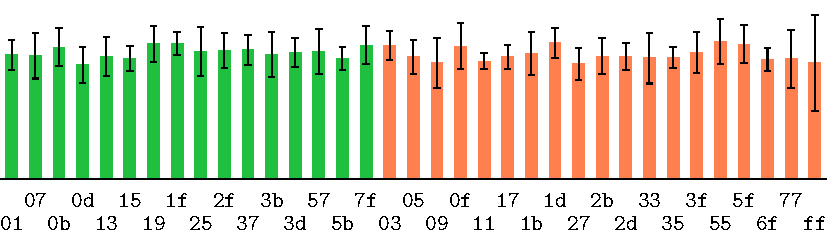
\includegraphics{figures/leak_target/leak_target.pdf}
		\caption{Success rate by targets' corresponding $p$'s and their standard deviation. Green represents invertible $p$'s, orange noninvertible ones.}
		\label{fig:leaktargethist}
	\end{center}
	\end{figure}
	
	%~ Note high deviation at {\tt ff}, this is because there is only a single target in this group (one generated by $B^T = (1,1,1,1,1,1,1,1)$).   %!% totál blbost, dev se přece nemůže zlepšovat počtem měření ne?
	Note that we did not give $y$-axis scale since the purpose is only to distinguish uniform distribution.
	
	\paragraph{Group with fixed $4$ bits in $B$.}
	
	Another way of grouping we performed, groups targets by fixing $4$ out of $8$ bits of their corresponding vector $B$, see Equation \ref{eq:tba}. We fixed the first and the last $4$ bits and grouped them, see results in Figure \ref{fig:leaktargetotherhist}, where these ways of grouping are in green or orange, respectively. Group index can be computed as binary AND of mask {\tt 0xf0} or {\tt 0x0f} with vector $B$, respectively.
	
	\begin{figure}[h]
	\begin{center}
		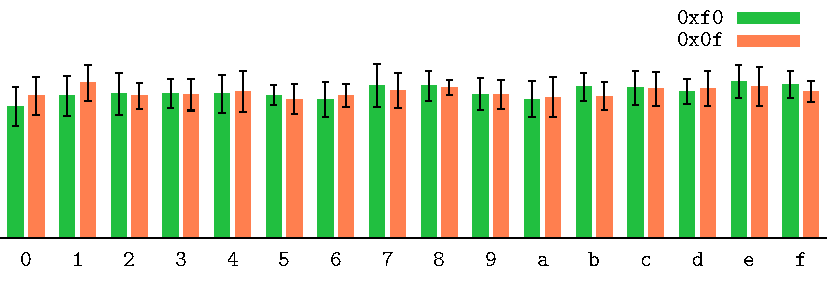
\includegraphics{figures/leak_target_other/leak_0x0f_0xf0.pdf}
		\caption{Success rate by fixed $4$ bits of targets' corresponding vector $B$. Green represents fixed first $4$ bits, orange represents last $4$ bits.}
		\label{fig:leaktargetotherhist}
	\end{center}
	\end{figure}
	
	\begin{remark}
	\label{rem:uniform}
		According to our observations, there does not seem to be a preferred target or a group of targets, therefore we will assume that target success rate is constant across all targets.
	\end{remark}

\subsubsection{False Positives}
	
	There is an inconvenience which emerges once we do not know the key -- we do not recognize the correct candidate anymore (see Remark \ref{rem:false}). Therefore we observed behavior of the incorrect ones.
	
	\paragraph{Gaps of incorrect candidates.}
		
		Previously we defined a strong candidate as a candidate with a gap larger than $10\%$. Most candidates which exceeded this limit were also correct candidates, but there were a couple of exceptions which we will refer to as {\em false positives}. Note that $25\%$ of candidates were strong and correct, on the other hand, there were $11\%$ of strong and incorrect ones. On average, strong incorrect candidates had a gap of $14\%$ (cf.\ $40\%$ for correct ones) and the highest gap ever seen was $35\%$ (cf.\ $76\%$ for correct ones). We need another observation about incorrect candidates in order to distinguish them from the correct ones.
		% 1024:
		% strong & correct:
		% 	[1019, 1000, 978, 1008, 986, 1006, 1019, 999] => 1001.875 ... 24.6%
		% 	[39.46, 39.68, 39.5, 40.28, 40.2, 39.85, 39.86, 39.68] => 39.81375
		% strong & incorrect:
		% 	[442, 440, 425, 415, 433, 463, 413, 468] => 437.375 ... 10.7%
		% 	[14.05, 14.06, 14.16, 13.95, 14.26, 13.83, 14.0, 13.97] => 14.035
	
	\paragraph{Number of repetitions of strong incorrect candidates.}
		
		The good news is that incorrect candidates do not repeat among targets very often. We observed the number of most repeating strong incorrect candidates among our $255$ targets and got following results: on average, the number was $1.75$, the maximum was $3$.
		% 	[1.88, 1.75, 1.81, 1.81, 1.62, 1.88, 1.62, 1.62]

\subsubsection{Using Less Traces}
	
	So far we used $1024$ traces in our attack, let us have a look at results of the attack with much less traces. Note that Bos et al.\ \cite{bos2015differential} used $2000$ and $500$ traces for the attack targetting the original SBox and Rijndael inverse, respectively.
	
	We used also much less traces, namely $128$, $256$, $384$ and $512$. For each number of traces we attacked all of our $8$ instances of {\tt KlinecWBAES} and observed success rate of strong candidates and their average gap. See results in Table \ref{tab:ntraces}.
	
	\begin{table}[h]
		\begin{center}
		\begin{tabular}{| c | c | c | c | c | c | c | c |}
			\hline
			Traces       &    $128$ &    $256$ &    $384$ &    $512$ &    $1024$ \\
			\hline
			Success rate &  $9.8\%$ &   $17\%$ &   $20\%$ &   $21\%$ &    $25\%$ \\
			\hline
			Average gap  &   $24\%$ &   $32\%$ &   $35\%$ &   $37\%$ &    $40\%$ \\
			\hline
			Reduced cost\footnote{Will be introduced later.}
			             & $5\,400$ & $4\,700$ & $5\,500$ & $6\,400$ & $10\,500$ \\
			\hline
		\end{tabular}
		\end{center}
	\caption{Success rates and average gaps using different numbers of traces.}
	\label{tab:ntraces}
	\end{table}
	
	% 128:
	% strong & correct:
	% 	[388, 420, 391, 411, 402, 393, 412, 397] => 401.750 ... 9.8%
	% 	[24.23, 24.39, 24.26, 23.65, 24.5, 24.01, 23.87, 23.65] => 24.07
	% strong & incorrect:
	% 	[262, 325, 351, 322, 309, 342, 285, 315] => 313.875 ... 7.7%
	% 	[13.34, 13.34, 13.13, 13.12, 12.9, 13.22, 13.26, 13.33] => 13.205
	
	% 256:
	% strong & correct:
	% 	[700, 670, 658, 722, 700, 709, 707, 683] => 693.625 ... 17.0%
	% 	[31.74, 32.49, 32.41, 31.83, 32.29, 31.31, 31.91, 32.11] => 32.01125
	% strong & incorrect:
	% 	[431, 472, 423, 441, 447, 451, 424, 482] => 446.375 ... 10.9%
	% 	[13.82, 13.85, 13.69, 14.1, 14.01, 14.1, 13.95, 14.36] => 13.985
	
	% 384:
	% strong & correct:
	% 	[814, 791, 784, 825, 790, 819, 812, 818] => 806.625 ... 19.8%
	% 	[35.84, 35.59, 35.14, 35.26, 36.19, 35.26, 35.77, 34.61] => 35.4575
	% strong & incorrect:
	% 	[491,488,484,504,487,464,509,530]
	% 	[14.17,14.37,13.97,14.17,14.14,14.07,14.23,14.30]
	
	% 512:
	% strong & correct:
	% 	[879, 851, 855, 887, 848, 879, 881, 870] => 868.75 ... 21.3%
	% 	[37.25, 37.47, 36.58, 37.66, 38.04, 37.03, 37.42, 36.93] => 37.2975
	% strong & incorrect:
	% 	[471,480,473,478,472,517,432,474]
	% 	[14.02,14.09,13.96,13.97,14.23,13.71,14.29,13.97]

\subsubsection{Leaking Bits}
	
	Remind that our trace is a bit-wise serialization of least significant bytes of memory addresses, hence we can identify which bit within that byte leaked -- simply by taking the leaking position within trace modulo $8$. This moduled position will be referred to as {\em leaking bit} (note the difference from target bit).
	
	We noticed soon that leaking bits are not very well balanced (as one would expect), therefore we put this data into a histogram, see Figure \ref{fig:leakbitall}. The histogram shows the amount of correct candidates with a gap larger than $10\%$ averaged over $8$ WBAES instances, for each leaking bit, together with standard deviation which is surprisingly very low. Note that the histogram does not provide absolute values since these could be misleading, only distribution is relevant at the moment.
	
	\begin{figure}[h]
	\begin{center}
		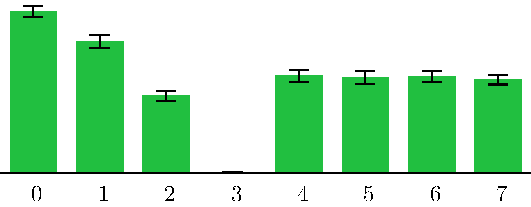
\includegraphics{figures/leak_bit/leak_bit.pdf}
		\caption{Average number of leaks and its standard deviation at each bit within trace.}
		\label{fig:leakbitall}
	\end{center}
	\end{figure}
	
	The \nth{0} and \nth{1} bits leaked slightly more, the \nth{2} bit slightly less and the \nth{3} bit actually leaked only twice while the overal average of the remaining bits was almost $160$! On the other hand, all of the remaining bits leaked fairly similarly. We do not have any explanation for this behavior.


% ==============================================================================
% ===   B L I N D   A T T A C K   S U G G E S T I O N                        ===
% ==============================================================================

\subsection{Blind Attack Suggestion}
\label{sec:subblindattack}

\begin{note}
	This section only applies previous observations on a heuristic basis, there is no guarantee that our approach is the best.
\end{note}

In general, we suggest to use rather less traces and repeat the attack with several targets until the sum of strong gaps of any candidate exceeds given bound.

In order to figure out a reasonable number of traces from results in Table \ref{tab:ntraces}, we introduce {\em reduced cost of gap}, defined as
\begin{equation}
\label{eq:redcost}
	C(n, s, g) = \frac{n}{s\cdot g} ,
\end{equation}
where $n$ stands for the number of traces, $s$ for average success rate and $g$ for average gap of a strong candidate.

%?% omitting strong candidates' bound leads to ~1.5\% enhancement
Note that this quantity corresponds with average time of the attack: the more traces, the longer time; the better success rate or the bigger gap, the shorter time. Thus we can use this measure to compare expected time of the attack using different number of traces. According to results in Table \ref{tab:ntraces}, the best value of the reduced cost of gap was achieved for $256$ traces, therefore we suggest to use this amount of traces.

As stated before, %!% where?
false candidates do not appear to repeat very much, the same situation was with $256$ traces. Therefore we suggest to keep using $75\%$ as a cummulative bound.

Note that we could perform an adaptive attack: start with lower cummulative bound, get some key candidate, verify it, and unless correct, keep increasing the cummulative bound while keeping the previous results. However, we did not implement this enhanced variant.
% vyzkoušet jestli tak zlomim všechny instance

% psal já / Teuwen:
%~ > I only wonder about the reasoning why Karroumi is more than Chow since
%~ > it seems to have been shown to be equal (based on what I wrote in my
%~ > previous email).
%~ 
%~ Well I've no problem to break completely Chow with standard DCA so there
%~ is something a bit more in Karroumi. Obviously not enough to make it
%~ robust enough...
